\documentclass[12pt,fleqn]{article}\usepackage{../common}
\begin{document}
Ders 1

Bir vektor 1) yon 2) buyukluk (magnitude) bilgisini tasiyan bir olcumdur. 

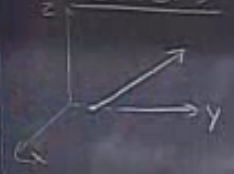
\includegraphics[height=2cm]{1_1.png}

Uc boyutlu bir ortamda x,y,z eksenleri uzerinden ustteki gibi bir vektor
cizebilirdik. Bu vektor (ok istikametinde) bir yonu gosteriyor, bir
buyuklugu de var. Vektoru bu eksenler icinde cizince, o vektoru her
eksendeki yansimasina gore temsil edebilirim demektir; x yonunde ne kadar
degisim var, y yonunde ne kadar var, vs. gibi.

Sembolik olarak harfin uzerinde bir ok isareti, mesela $\vec{A}$ gibi, bize
elimizdeki degiskenin bir vektor oldugunu hatirlatmak icindir. Bazi
kitaplarda ok yerine sembol sadece koyu renkli olarak gosterilmis olabilir,
bunu tarihi sebepleri var, cunku matbaa baskisinda eskiden koyulugu (bold)
yapmak kolaydi, ok isaretini yapmak zordu. 

Bir vektoru birim vektorler uzerinden temsil etmek mumkundur, mesela 

\[ \vec{A} = a_1 \hat{i} + a_2 \hat{j} + a_3 \hat{k} \]

ki birim vektorler tek bir eksen uzerinde tek birimlik bir adimi temsil
ederler. Mesela $\hat{i}$, x ekseni uzerinde 1 adimlik bir buyukluktur,
digerlerinde degisim sifirdir, $\hat{i} = <1,0,0>$. Notasyonun isleyip
islemedigine bakalim, eger $<2,3,5>$ vektorunu temsil etmek isteseydik,
bunu $2\cdot<1,0,0> + 3\cdot<0,1,0> + 5\cdot<0,0,5>$ ile
yapabilirdik. Toplam $<2,3,5>$ verecekti. 

Hazir bahsetmisken, diger vektor notasyonu

\[ \vec{A} = <a_1, a_2, a_3> \]

Vektor buyuklugu $|\vec{A}|$ ile gosterilir, ki $|\cdot|$ isareti mutlak
deger (absolute value) notasyonu ile aynidir. Bu deger tek bir sayi
(scalar) geri getirir. Vektor yonu, ki bu bazen $dir(\vec{A})$ ile
gosterilir, vektorun birim vektor haline getirilmesi ile elde edilir, yani
vektorun tum ogelerinin onun buyuklugune bolunmesi ile. Bu yapilinca vektor
buyukluk bilgisi kaybolmus olur tabii, geriye sadece yon kalir. Bu bilgi,
daha dogrusu, ``sadece yon'' verisi icerir, yoksa vektor oldugu sekliyle de
yon bilgisini zaten icerir.

Iki nokta $P$ ve $Q$ arasinda bir vektoru $\vec{PQ}$ olarak
gosterebilirim. Fakat bu illa ki $P$'den baslayip $Q$'ye gelmem gerektigi
anlamina gelmez, ayni yonde ayni uzunlukta paralel bir baska vektor de
$\vec{PQ}$ vektoru olabilir. Bu derste pek cok vektoru orijin noktasindan (0,0,0)
baslayarak cizecegiz, fakat aslinda bunu yapmak mecburi degil. Cizimsel
basitlik icin bunu yapacagiz. 

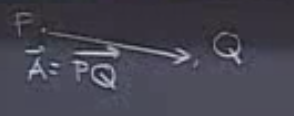
\includegraphics[height=2cm]{1_2.png}

Simdi alttaki grafige bakalim. Uzunluk nedir?

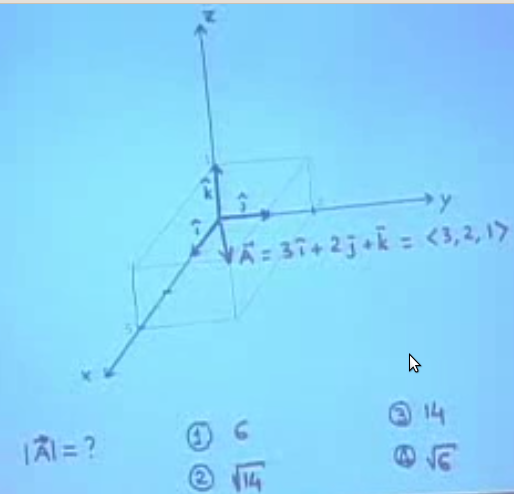
\includegraphics[height=6cm]{1_3.png}

Yani $\vec{A} = <3,2,1>$'in uzunlugu nedir?  Bu uzunlugu bulmak icin ikinci bir
resme bakalim:

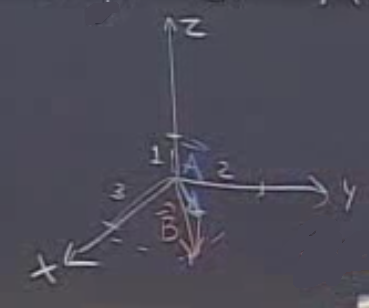
\includegraphics[height=4cm]{1_4.png}

Burada $\vec{A}$'nin yz duzlemine olan yansimasini $\vec{B}$ olarak
dusunelim, $\vec{A}$ sadece xy degerlerini tasiyor yani $\vec{B} = <3,2>$.
Simdi $\vec{A}$ ve $\vec{B}$'nin ikisinin de uzerinde oldugu ve bir tarafi
z ekseni olan bir kesiti hayal edelim. Bu kesiti ayirip alttaki gibi
cizebiliriz:

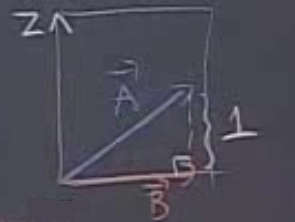
\includegraphics[height=3cm]{1_5.png}

Goruldugu gibi $\vec{A}$ ve $\vec{B}$ arasinda z baglaminda 1 birimlik bir
fark var, bu da $\vec{A} = <3,2,1>$ vektorunu $\vec{B}=<3,2>$ olarak
alirken dahil etmedigimiz 1 degeri.

Ustteki grafige bakarsak Pitagor teoresini kullanarak $|\vec{A}|$'yi
bulabiliriz. $|\vec{A}|^2 = |\vec{B}|^2 + 1^2$. Demek ki problem
$|\vec{B}|$'nin hesaplanmasina indirgendi,cunku onu bulursak ustteki
formulden $|\vec{A}|$'yi da bulabiliriz. $|\vec{B}|$ nedir? Onu da xy
duzleminde / kesitinde Pitagor kullanarak bulabiliriz, $|\vec{B}|$ x
ekseninde 3 birim, y ekseninde 2 birimlik adimlar iceriyor, Pitagoru
kullanirsak

\[  \vec{B} = \sqrt{3^2 + 2^2} = \sqrt{13} \]

\[ |\vec{A}| = \sqrt{|\vec{B}|^2 + 1^2} = \sqrt{13 + 1} = \sqrt{14} \]

Genel formul

\[ |\vec{A}| = \sqrt{a_1 ^2 + a_2^2 + a_3^2} \]

Vektorlerle baska ne yapabiliriz? Onlari ekleyebiliriz, ve
olcekleyebiliriz. 

Ekleme

Elimizde $\vec{A}$ ve $\vec{B}$ var ise, $\vec{A} + \vec{B}$ hesabini yapabiliriz. 

Bu noktada su yorumu eklemek gerekir, vektorler iki farkli dunyada
yasarlar, bir tanesi geometrik dunya (sekilsel), digeri hesapsal dunya
(sayilarla temsilleri). Bu sebeple vektorler hakkindaki her sorunun iki
cevabi vardir, biri geometrik digeri sayisal cevap.

Geometrik cevap ile baslayalim: 

Diyelim ki iki vektoru ayni noktadan cikacak sekilde cizmistim

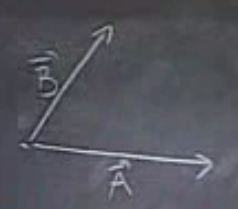
\includegraphics[height=2cm]{1_6.png}

Toplami almak icin $\vec{B}$'yi alip hareket ettiririm (baslangic bitis
noktalarinin onemli olmadigini soylemistik), ve $\vec{A}$'nin bittigi
noktadan baslamasini saglarim.

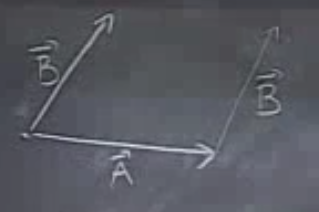
\includegraphics[height=2cm]{1_7.png}

Bunun bir paralelogram ortaya cikardigini goruyoruz. 

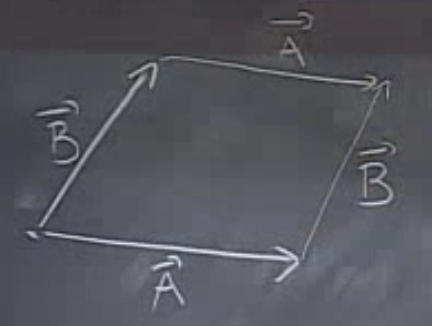
\includegraphics[height=2cm]{1_8.png}

Eger bu paralelogramin caprazini hesaplarsak / cizersek, iste bu capraz
$\vec{A} + \vec{B}$ olarak nitelenebilir. 

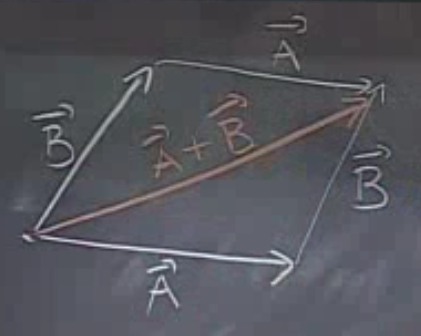
\includegraphics[height=2cm]{1_9.png}

Yani bu iki vektorun birbiriyle toplanmasi $\vec{A}$ uzerinde, sonra
$\vec{B}$ uzerinde hareket etmekle esdeger. Ya da, paralelogramin ust
kismina bakarsak, once $\vec{B}$ sonra $\vec{A}$ yonunde hareket etmekle
esdeger ($\vec{A} + \vec{B} = \vec{B} + \vec{A}$ esitligini grafiksel
olarak boylece dogrulamis ta olduk).

Sayisal olarak dusunursek

\[ \vec{A} = <a_1, a_2, a_3> \]

\[ \vec{B} = <b_1, b_2, b_3> \]

\[ \vec{A} + \vec{B} = <a_1+b_1, a_2+b_2, a_3+b_3> \]

Tek Sayi Ile Carpmak

Eger elimizde $\vec{A}$ var ise, $2 \cdot \vec{A}$ ile bu vektoru ayni
yonde iki kat daha fazla gitmesini saglayabiliriz. Ya da yarisi, ya da eksi
yonde, vs.

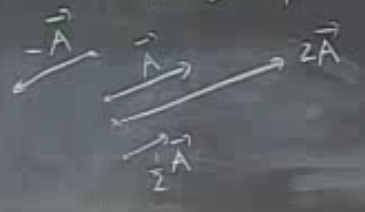
\includegraphics[height=2cm]{1_10.png}

Simdi vektorler hakkinda birkac yeni operasyon daha ogrenecegiz. Bu
operasyonlar geometriye daha detayli sekilde baslayinca isimize
yarayacak. Ileride gorecegimiz gibi, geometri vektorler uzerinden
yapilabilir, hatta pek cok acidan, geometri de calismak icin vektorlerin
``en uygun dil'' oldugu soylenebilir. Ozellikle fonksiyonlar konusuna
gelince vektorler kullanmak, diger tur geometrik islemleri kullanmaktan
daha faydali olacak. 

Tum bunlar bir tur ``dil'', bir seyin farkli bir sekillerde temsilinden
ibaret, vektorler, fonksiyonlar, vs. gibi temsili objeler. Fakat notasyon
fark yaratabiliyor, bazi seyleri kolaylastirip, temizlik getirebilmesi
acisindan.

Noktasal Carpim 

\begin{equation}\label{eq1}
\vec{A} \cdot \vec{B} = \sum a_ib_i = a_1b_1 + a_2b_2 + a_3b_3 
\end{equation}

Onemli bir nokta: Sonuc bir tek sayi (scalar), bir vektor degil. 

Peki bu operasyon niye kullanilir? Neye yarar? Aslinda biraz garip bir
operasyon. Bu sorunun cevabini vermeden once belki de geometrik olarak ne
yaptigini gostermek daha iyi olur. Iddia ediyorum ki

\begin{equation}\label{eq2}
\vec{A} \cdot \vec{B} = |\vec{A}||\vec{B}| \cos \theta 
\end{equation}

ki $\theta$ iki vektorun arasindaki aci

Fakat dedigimiz gibi, bu operasyon cok suni bir sey gibi duruyor. Niye bu
cetrefil operasyonu yapalim ki? Su sebepten: elde ettigimiz sonuc,
$|\vec{A}||\vec{B}| \cos \theta $ esitligi uzerinden bize hem buyuklukler
baglaminda, hem de acisal baglamda bir seyler soyluyor / bilgi
veriyor. Ekstra bir bonus ise bu hesabin cok kolay yapilabilmesi, iki
vektorun ogelerini teker teker birbiriyle carpinca noktasal carpim sonucunu
elde ediyoruz. 

Fakat noktasal carpim ve buyukluk, aci iceren formul arasinda ne baglanti
var? Matematikte bu tur baglantilarin ispatlanmasi gerekir. Ustteki esitlik
bir teoridir (bu dersin ilk teorisi!). Ispatlayalim. Icinde buyukluk ve aci
iceren geometrik tanim ne anlama geliyor? Alttaki ifade uzerinden kontrol
edelim. Eger $\vec{A}$'nin kendisi ile noktasal carpimini alsak ne olurdu?

1) $\vec{A} \cdot \vec{A} = |A|^2cos(0) = |A|^2$

$cos(0)$ cunku vektorun kendisi ile noktasal carpimini aliyoruz, vektorun
kendisi ile arasindaki aci sifir. Sifirin cos degeri 1. Peki diger formu
kullansaydik ne olacakti? O zaman

\[ a_1^2 + a_2^2 + a_3^2 \]

elde edecektik, ki bu ifade $|A|^2$'ye esittir cunku buyuklugun tanimini
hatirlarsak

\[ |\vec{A}| = \sqrt{a_1 ^2 + a_2^2 + a_3^2} \]

iki tarafin karesini alirsak

\[ |\vec{A}|^2 = a_1 ^2 + a_2^2 + a_3^2\]

bu ifadenin sag tarafi noktasal carpimdan elde ettigimizle ayni. 

2) Peki ya elimizde iki farkli vektor varsa? 

Iddiam su ki formul \ref{eq1} ve \ref{eq2} arasindaki iliskiye Kosinus
Kanunu ile kurabilirim. Bu kanunu yazalim

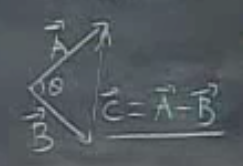
\includegraphics[height=2cm]{1_11.png}

\[ |\vec{C}|^2 = |\vec{A}|^2 + |\vec{B}|^2 - 2|\vec{A}||\vec{B}|cos(\theta) \]

Bu arada, eger bu formulu 

\[ |\vec{C}|^2 = |\vec{A}|^2 + |\vec{B}|^2  \]

seklinde yazsaydim Pitagor Formulu olurdu, ama burada Pitagor kullanamayiz
cunku arada dik aci yok, o yuzden ucuncu terimi eklemek gerekti. 

Ispat

Soyle baslayalim

\[ |\vec{C}|^2 = \vec{C} \cdot \vec{C} \]

Bunun dogru oldugunu biliyoruz, daha once ispatladik. $\vec{C}$'nin
ustteki tanimini yerine koyarsak

\[ = (\vec{A} - \vec{B}) \cdot (\vec{A} - \vec{B})  \]

Simdi bu carpimi acarak 4 terimin toplami haline getirmek isterdik, ama
bunu yapabilir miyiz? Daha bilmiyoruz, noktasal carpim operasyonunu daha
yeni gorduk, gizemli yeni bir operasyon bizim icin su anda. Fakat cevap
evet, cunku formul \ref{eq1}'deki tanima bakarsak, acilim yapmak icin bize
gerekli sekilde davranacagini gorebiliriz. O zaman

\[  =
\vec{A}\cdot\vec{A} - 
\vec{A}\cdot\vec{B} -
\vec{B}\cdot\vec{A} +
\vec{B}\cdot\vec{B} 
\]

Ilk ve son terimin karsiligini hemen yazabiliriz, alttaki ilk iki terim
onlar zaten

\[ = |\vec{A}|^2 + |\vec{B}|^2 - 2\vec{A} \cdot \vec{B} \]

Geride kalan en son terimi, son formul icindeki cos iceren formul ile
karsilastiralim, aralarindaki tek fark, bir tarafta $2\vec{A} \cdot
\vec{B}$ diger 
tarafta $2|\vec{A}||\vec{B}|cos(\theta)$ olmasi.. Ve formul \ref{eq2}'deki 
esitlikten  bu iki terimin de aslinda birbirine esit oldugunu
biliyoruz. 

Uygulamalar

1) Uzunluklari ve acilari (ozellikle acilari) hesaplamak.

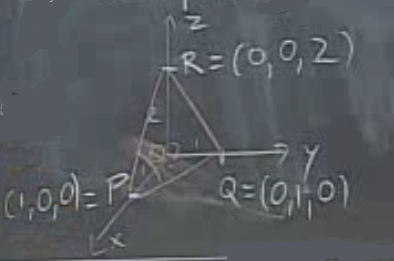
\includegraphics[height=4cm]{1_12.png}

Diyelim ki sol alt kosedeki $\theta$ acisini hesaplamak istiyoruz. 

\[ \vec{PQ} \cdot \vec{PR} = |\vec{PQ}||\vec{PR}|cos(\theta)  \]

Bu formulde bilinmeyen $\theta$, bilahere $cos(\theta)$. Uzunluklari
hesaplayabiliriz, formulunu biliyoruz. Noktasal carpimlari da
hesaplayabiliriz, onun da basit bir formulu var. 

\[ \cos\theta = \frac{\vec{PQ} \cdot \vec{PR}}{|\vec{PQ}||\vec{PR}|}\]

\[ = \frac{<-1,1,0>\cdot<-1,0,2>}
{  \sqrt{(-1)^2+1^2+0^2 }\sqrt{(-1)^2+0^2+2^2 }   } 
\]

\[ = \frac{1+0+0}{\sqrt{2}\sqrt{5}}  \]

\[ = \frac{1}{\sqrt{10}} \]

\[ \theta = \cos^{-1}(\frac{1}{\sqrt{10}}) \approx 71.5^o \]

Burada $\vec{A}\cdot\vec{B}$'nin isaretine (arti mi eksi mi) dikkat
cekelim. 

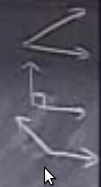
\includegraphics[height=4cm]{1_13.png}

Eger isaret $>0$ ise, o zaman $\theta < 90^o$ (ustteki resimdeki
1. figur). 

Eger isaret $=0$ ise, o zaman $\theta = 90^o$ (ustteki resimdeki
2. figur). 

Eger isaret $<0$ ise, o zaman $\theta > 90^o$ (ustteki resimdeki
3. figur). 

Yani noktasal carpim bir nevi iki vektorun ne kadar ``beraber gittigini''
olcuyor. Ustte 1. sekil asagi yukari ayni yone dogru giden iki vektor, ve
isaretleri pozitif. 2. sekil dikine giden vektorler, alaka yok. Tersine
gidenlerde isaret negatif. 

2) Diklik Kontrolu

Diyelim ki size 

\[ x + 2y + 3z = 0 \]

seklinde bir formul verdim. Sizce bu formul nasil bir sekle sebebiyet
verir? Cevaplar:

\begin{enumerate}
   \item Bos kume (cozum yok)
   \item Tek bir nokta
   \item Bir cizgi
   \item Bir duzlem
   \item Bir kure (sphere)
   \item Usttekilerin hicbiri
   \item Bilmiyorum
\end{enumerate}

Dusunun.. 

Dogru cevap: 4. 

Bunun bir duzlem oldugunu nasil gorebiliriz? Vektorler burada yardimimiza
yetisiyor. Bir $\vec{OP}$ vektoru oldugunu dusunelim, ki bu vektorun
ogeleri $x,y,z$ olsun. 

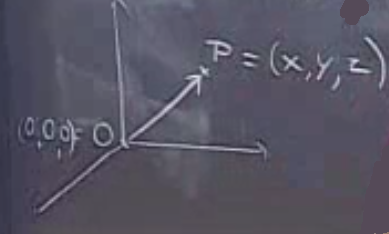
\includegraphics[height=4cm]{1_14.png}

$x + 2y + 3z = 0$ ifadesine bakarsak, onu bir noktasal carpim olarak temsil
edebiliriz, bu carpim $\vec{OP}$ ile ``bir baska vektorun'' carpimi
olabilir. Bu diger vektor $\vec{A} = <1,2,3>$ vektoru olabilir. O zaman su kosul

\[ x + 2y + 3z = 0 \]

Aslinda

\[ \vec{OP} \cdot \vec{A} = 0 \]

olarak ta temsil edilebilir.

Peki ustteki noktasal carpimin sifira esit olmasi ne demektir? Vektorler
hakkindaki bilgilerimizi kullanirsak, sifira esitlik bu iki vektorun
birbirine dik olmasi anlamina gelir. O zaman duzlemin ne oldugu hakkinda
bir ek bilinc daha gelistirmis olduk. Elde ettigimiz orijin noktasindan
gecen bir duzlem ve $\vec{A}$'ya dik. 

Fakat elimize gecen ozgun / tekil (unique) bir duzlem mi yoksa
seceneklerden sadece biri mi? Cunku su akla gelebilir: eger bir vektor
baslangic olarak herhangi bir yere konulabiliyorsa, o zaman herhangi bir
yerden baslayabilecek $<1,2,3>$'ye dik olmak ne demektir? 

Iyi bir soru fakat sunu hatirlayalim: Baslangic degisse de yon degismiyor,
yani farkli duzlemler olsa bile birbirlerine paralel olurlar. Ayrica $x +
2y + 3z = 0$ 
formulune iyi bakalim, bu formulu tatmin eden pek cok $x,y,z$
degerlerinden birisi $0,0,0$ degeridir, yani orijin noktasidir. O zaman bu duzlem
orijinden kesinlikle gecmeli, ki bu mumkun duzlemleri tek bir secenege
indiriyor. 

Duzlem formulu $ax + by + cz + d= 0$ diye gider, bizim formulde $d=0$. Bu
form orijinden gecme zorundadir.

Bu duzlemi grafiklemek icin alttaki programi kullanalim

\begin{minted}{python}
# plotting ax + by + cz = 0, or (ax + by)/-c  = z 
# ax + by + cz = 0 formulu grafikliyoruz ya da, (ax + by)/-c  = z 

from mpl_toolkits.mplot3d import Axes3D
import matplotlib.pyplot as plt
import pylab as p

fig = plt.figure()
ax = Axes3D(fig)
X = np.arange(-10, 10, 0.5)
Y = np.arange(-10, 10, 0.5)
X, Y = np.meshgrid(X, Y)

Z = (X + 2*Y ) / -3

surf = ax.plot_surface(X, Y, Z,rstride=1, cstride=1, alpha=0.3)

ax.set_xlim3d(-10, 10)
ax.set_ylim3d(-10, 10)
ax.set_zlim3d(0, 30)

plt.savefig('plane.png')
\end{minted}

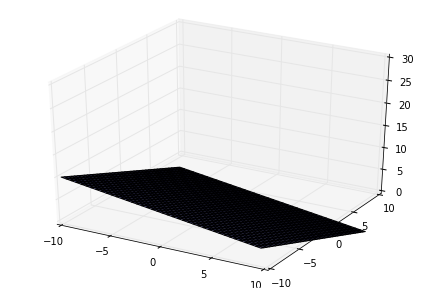
\includegraphics[height=6cm]{plane.png}

\end{document}
